\chapter{Introduction}
\label{chapter:Intro}

Blockchain technology has seen an enormous rise in interest in the recent years, coming to its climax at the end of 2017. The driving factor behind this is 1) Bitcoin, the most known cryptocurrency in the market and 2) 
Linear to the rising interest, articles trying to explain what lies behind the name have popped up in the thousands. Simple Google search requests for "what is bitcoin" and "what is blockchain" have peaked in December 2017, see figure \ref{fig:SearchRequests}, and yield 10.6 million and 3.8 million results. Of these results, the top ones claim to explain the technology in as little words as possible ("WTF is The Blockchain?
The ultimate 3500-word guide in plain English to understand Blockchain.",\footcite{MamoriaWTFBlockchain2017}, "Explain Bitcoin Like I'm 5"\footcite{CustodioExplainBitcoinFive2013}, "Blockchain: everything you want to know about the technology but were too embarrassed to ask"\footcite{HeathmannBlockchaineverythingyou2018} or "Still don't understand the blockchain? This explainer will help"\footcite{LeighSinodStilldonunderstand2018}) The internet offers A LOT of resources to learn about blockchain and the cryptocurrencies that build on top, but most of these articles only cover the very basics of the technology and do not point out its limits, thus (maybe unconsciously) taking part in causing the hype. Many (including big consulting companies such as Deloitte) claim that blockchain has dozens of potential applications in almost every major industry, (financial services, technology, media, and telecommunications, consumer and industrial products, life sciences and health care, public sector, energy and resources and horizontal applications(e.g. audit and cyber security)).\footcite{SchatskybitcoinBlockchaincoming2015} These claims are picked up from a hyped up management that not fully understands the technology and yet wants to utilize it -> because Hype.

\begin{figure}
    \centering
    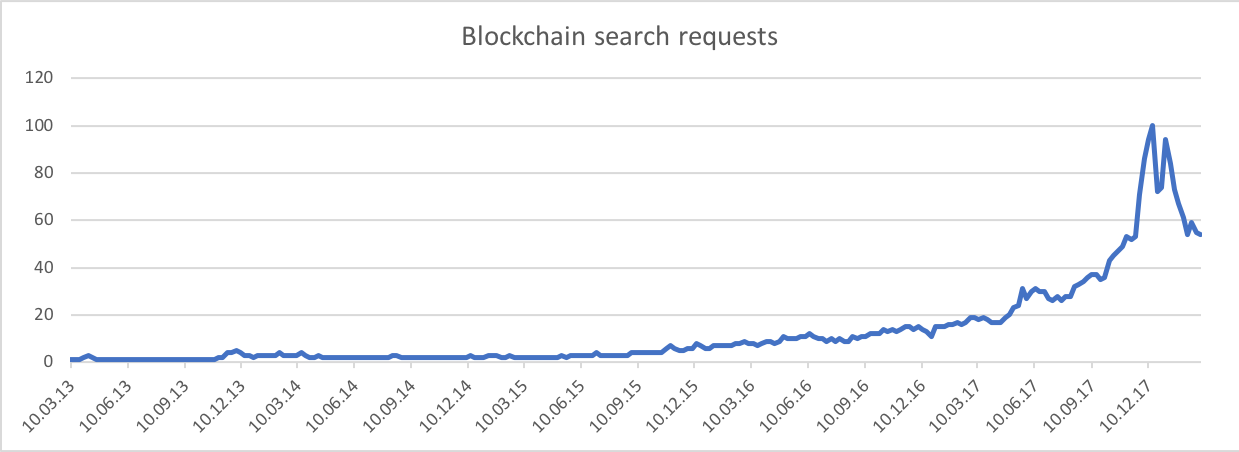
\includegraphics[width=\textwidth]{latex-vorlage_v1.5/graphics/BCRQ.png}
    \caption[Google Trends results for "blockchain" search requests.]{Google Trends results for "blockchain" search requests.\footnote{Data extracted on the 12th of March, 2018 from https://trends.google.com/trends/explore?date=today\%205-y\&q=\%2Fm\%2F0138n0j1
}}
    \label{fig:SearchRequests}
\end{figure}
%\footnotetext{Data extracted on the 12th of March, 2018 from https://trends.google.com/trends/explore?date=today\%205-y\&q=\%2Fm\%2F0138n0j1}

"Writing a description for this thing for general audiences is bloody hard. There's nothing to relate it to."\footcite{NakamotoReSlashdotSubmission2010}

https://moguldom.com/14060/100-of-the-best-quotes-on-bitcoin-and-blockchain/
“Every informed person needs to know about Bitcoin because it might be one of the world’s most important developments.”

–Leon Luow, Nobel Peace prize nominee 
\section{Problem statement} \label{sec:Problem}

The problem with this is however that many people suffer from the hype and solely want to establish a blockchain in their enterprise to show off. But in many cases, a blockchain is not necessarily the best option. This insight is quickly uncovered, if one deals with the topic a little more deeply than what most of the "what is blockchain" articles cover. Once one has reached a deeper level of understanding, blockchain's use cases are a lot more realistic and down-to-earth and one is aware of its limitations and where the technology is best applied. 

On the other hand, many people might be overwhelmed by the sheer mass of information/articles, that are out there regarding blockchain technology. One reason, as to why there are so many different attempts to explain the technology is because the authors feel that all the other articles do not correctly present the topic. The problem there is that the blockchain technology is indeed hard to explain, as it builds on a variety of different topics, such as cryptography, game theory, computer networking, data transmission as well as monetary theory.\footcite[Cf.][]{LoppNobodyUnderstandsBitcoin2017}

Show the motivation: Why is this topic important and interesting?

Describe the context of the problem: People don't understand blockchain and how transactions work, therefore they cannot imagine possible use cases as easily.

\section{Objective and scope} \label{sec:Objective}
\begin{itemize}
    \item Touch on the hype on Blockchain and take away the mystery/have people understand how it works and when it may be useful in order to not have inflated expectations.
    \item Say why I want to create an artifact to provide more details about blockchain technology
    \item Limit the scope of the research to only transactions (and one/a few selected coin/s(?))
    \item Articulate the research question that I want to explore in this thesis: How can blockchain transactions and smart contracts best be explained in a dashboard to persons that have only very limited knowledge about this topic?
    \item On basis of this research question, show which research method is going to be used for finding the answer.

\end{itemize}


    Objective should only be 2 to 3 sentences long!
    
    The study's research question is therefore: \textbf{What should the artifact visualize so it explains the blockchain technology in a comprehensible way?}
    
\section{Thesis overview} \label{sec:ThesisOverview}
How is this paper structured? What will be presented in the following chapters?


